\section{1. Introduction}
\subsection{1.1 Data wrangling is data analysis}

Data analysis is not only statistical analysis. Data analysis also includes data clean-up, transformation in and between data sets, visualization, and statistical analysis \parencite{Wickham2017R}. Yet, quantitative multilingual research often reports vague practices or fails to report any decisions made outside of statistical models, in part, because pre-processing software has already made the decisions for the researchers \parencite{Prystauka_Altmann_Rothman_2023}. These decisions, however, have pervasive implications across data analyses that affect replicability and reliability \parencite{ana_flex}. This is especially true for methods that capture real-time language processing, such as eye-tracking. Whereas open research practices, including shared data and code \parencite{Bolibaugh}, serve as a positive first step, the field still has a long way to go. 

\begin{figure}[h]
    \centering
    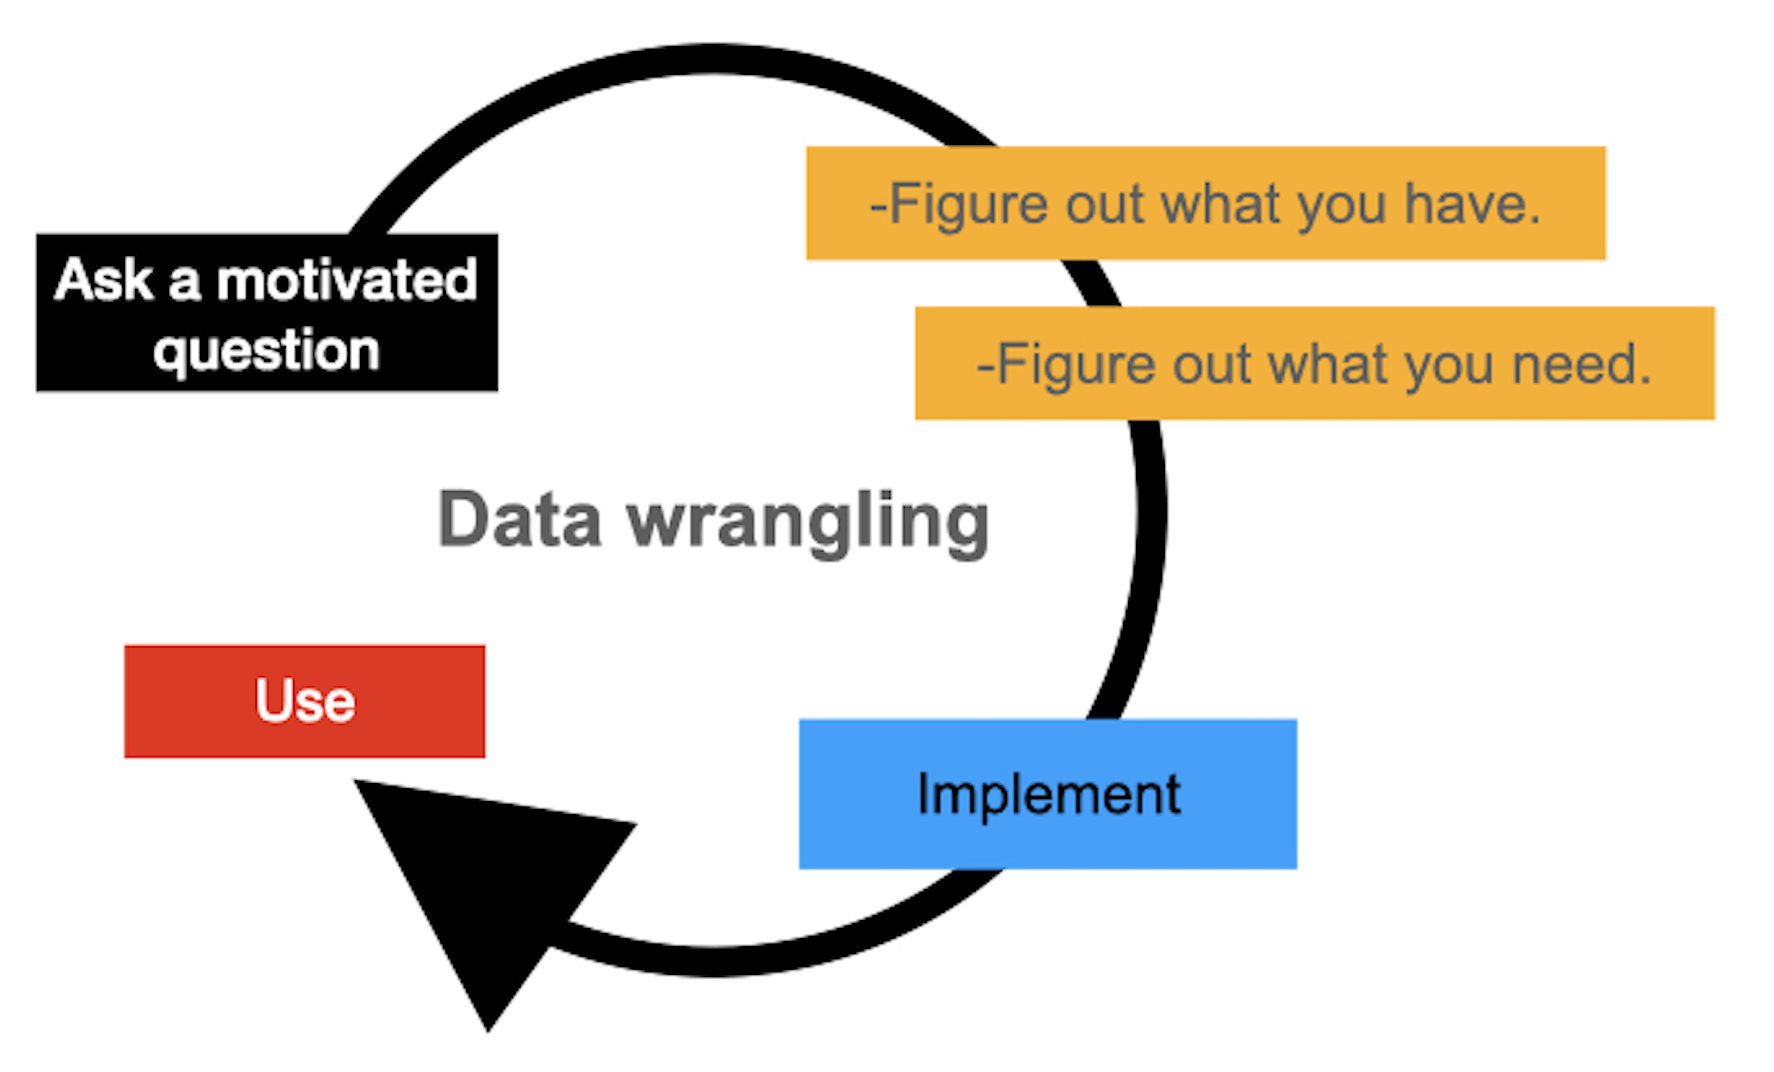
\includegraphics[scale=.3]{figures/data_wrangling.png}
    \caption{The data wrangling cycle: an iterative process including all steps, which reduce, reorder, extend, tidy, transform, and/or combine your data}
    \label{fig:data_wrangling}
\end{figure}

Here, we focus on data wrangling (see Figure \ref{fig:data_wrangling}); the iterative process of cleaning raw data straight from an experiment and transforming it into a usable structure (i.e., tidy data or data ready for visualization and statistical analysis) within a typical visual world paradigm eye-tracking study. Web-based eye-tracking has become more accessible and reliable than ever, capturing many effects found in in-person real-time processing experiments for a fraction of the cost \parencite[e.g.,][]{Vos_2017,Semmelmann_2017,Prystauka_Altmann_Rothman_2023,Degen_Seeing_2021}. However, access to these methods comes at the cost of requiring expertise in data wrangling \parencite[e.g., ][]{Vos_2017,Prystauka_Altmann_Rothman_2023}. Data from web-based experiments are currently even more complex than their in-person counterparts given the lack of subscriber-based pre-processing software, which means that the choices made during data wrangling are a new opportunity for radical open science practices. We present \textit{\textbf{The Art of Wrangling}} as a best practices guide for web-based eye-tracking using the lingua franca of data analytics, R \parencite{mizumoto_r_2015, R}. 
\newline
\newline